\documentclass[12pt]{article} 

\usepackage[latin1]{inputenc}
\usepackage[spanish]{babel}
\usepackage{color}
\usepackage{multicol}
\usepackage{amsmath}
\usepackage{amssymb}
\usepackage{enumerate}
\usepackage{graphics}
\usepackage{graphicx}


\title{COLAS}
\author{Sara Chica, Rodrigo Gualtero}
\date{10 de Noviembre, 2012}

\begin{document}
\maketitle
\tableofcontents

\section{Introducci�n}
Este es un problema de la UVA, identificado con el c�digo \textit{10128}, el cual consiste en encontrar el n�mero de posibilidades en que se pueden distribuir \textit{n} personas en una fila donde se ven \textit{l} cantidad de personas por el frente y \textit{r} por atr�s. Cada persona tiene una altura diferente, por lo tanto no deja ver a los m�s peque�os que est�n siendo ocultados por �l.
\\En los ejemplos que se encuentran a continuaci�n cada persona est� representada por una linea vertical.

\begin{center}
	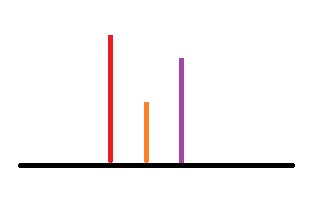
\includegraphics[width=0.50\textwidth]{Ejemplo1.jpg}
	\\Ejemplo 1.1: Hay 3 personas. Se ve por adelante 1 persona y por atr�s 2.
\end{center}
En el ejemplo anterior se puede ver que existe �na �nica posibilidad para que s�lo se vea 1 por adelante y 2 por atr�s y es la que se presenta.

\begin{center}
	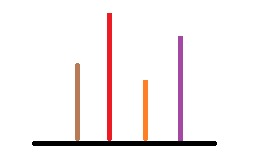
\includegraphics[width=0.50\textwidth]{Ejemplo2.jpg}
	\\Ejemplo 2.1: Hay 4 personas. Se ve por adelante 2 personas y por atr�s 2 tambi�n.
\end{center}
De estos se despliegan varias posibilidades, de las cuales 6 sirven.

\section{Definici�n del problema}
En este problema se desea encontrar las posibilidades para organizar \textit{n} cantidad de personas, de tal forma que tanto por delante como por atr�s se vea el mismo n�mero de personas que se plantea en la entrada. Es decir, si hay 3 personas, por delante se ve 1 persona y por detr�s 2, estos n�meros se deben conservar.
\subsection{Entrada}
Se recibe un n�mero entero que indica la cantidad de filas que entran \textit{(T)}.
\\De ah� en adelante entran T filas, cada una con 3 enteros, el primero la cantidad de personas que hay en la fila, el segundo cuantas personas se ven por delante y el tercero cuantas personas se ven por detr�s.
\subsection{Salida}
Por cada caso de prueba se debe imprimir una linea que contenga el n�mero de posibilidades que hay para organizar las personas de forma que se vea la misma cantidad por delante que anteriormente, lo mismo por atr�s. 

\section{Modelamiento matem\'atico}
Este problema se puede modelar como un �rbol de posibilidades donde cada fila es un nodo del �rbol, el cual a su vez tiene por dentro una tripla de 3 enteros $(n,l,r)$.

\begin{center}
	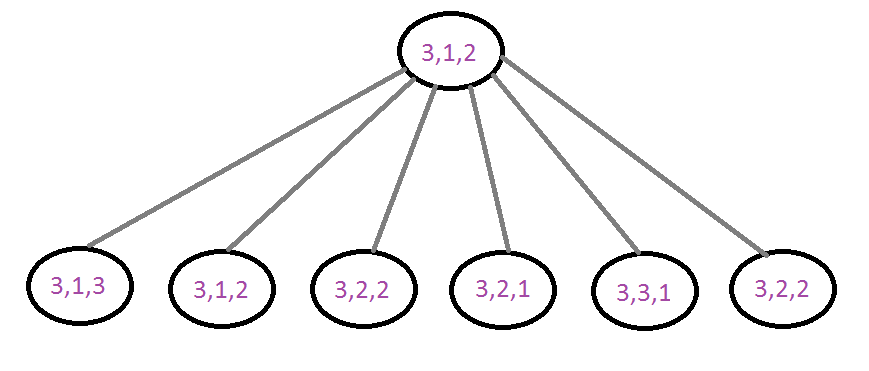
\includegraphics[width=0.50\textwidth]{Ejemplo1-2.png}
	\\Ejemplo 1.2: �rbol dado el ejemplo 1.1
\end{center}
Dado este �rbol se representa gr�ficamente el siguiente �rbol de posibilidades.
\begin{center}
	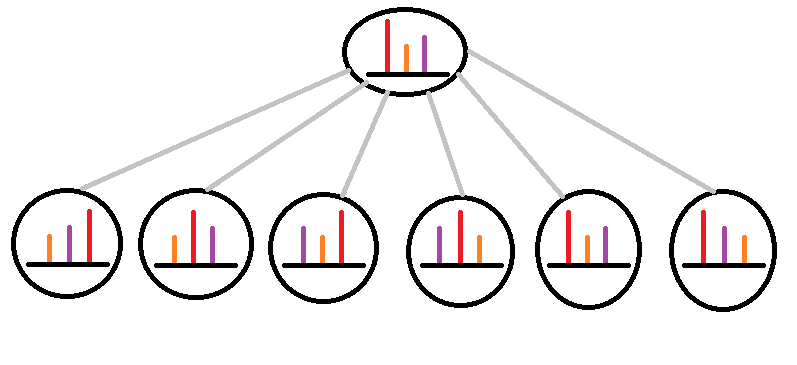
\includegraphics[width=0.50\textwidth]{Ejemplo1-3.png}
	\\Ejemplo 1.3: Representaci�n gr�fica de las posibilidades.
\end{center}

\section{Planteamiento de la Soluci�n}
Para determinar la soluci�n del problema se deben saber todas las posibles posibilidades para acomodar las personas y ver en ellas cuales son las que sirven para que se mantengan la misma cantidad de personas que se ven por el frente, como por atr�s.
\\En el ejemplo 1 se observa, abriendo el �rbol de posibilidades, que la �nica posibilidad para mantener las mismas cantidades es mantener las personas en el mismo lugar.
\\Llegar a la soluci�n ser�a posible de diferentes maneras, una de ellas por medio de backtraking, sin embargo existe otra forma para llegar a ella, se utilizan 3 \textit{for} anidados para realizar las diferentes permutaciones y obtener el resultado.

\section{Conclusiones}
\begin{enumerate}
	\item Backtraking permite obtener todas las permutaciones posibles, sin embargo utliza excesivamente los recursos, tales como memoria y tiempo, ya que tiene que abarcar cada una de las posilibidades.
	\item Por medio de los tipos de algoritmos de recorridos de �rboles se puede abarcar todas las posibilidades para solucionar un problema de este tipo, por lo tanto resulta importante conocerlos y saber como utilizarlos, as� de esta forma se llega a saber si es la mejor soluci�n o existe otra mejor.
\end{enumerate}
\end{document}